\documentclass[12pt]{article}
\usepackage[utf8]{inputenc}
\usepackage[margin=1in]{geometry}
\usepackage{float}
\usepackage{graphicx}
\usepackage{physics}
\usepackage{amsmath}
\usepackage{amssymb}
\usepackage[colorlinks]{hyperref}
\usepackage{subcaption}
\captionsetup{font=footnotesize}
\usepackage{booktabs}
\usepackage{multirow}
\usepackage{newtxtext, newtxmath}
\newcommand{\otoprule}{\midrule[\heavyrulewidth]}
\usepackage[export]{adjustbox}

\title{Dyakonov-Shur Instability in an Annulus}
\author{Jack Farrell}
\begin{document}
	\maketitle
	\section{Methods}
	\subsection{Equations}
	The domain is annulus of inner radius $R_1$ and outer radius $R_2$.  In conservation form (and also non-dimensional), the Navier-Stokes equation and continuity equation are:
	\begin{equation}
	\centering
		\begin{split}
			\pdv{\vb{J}}{t} + \div{\left( \vb{J} \otimes \frac{\vb{J}}{n}\right)} +\grad{n} = \eta \laplacian{\frac{\vb{J}}{n}} + \gamma (n\vb{v_0} - \vb{J}), \\
			\pdv{n}{t} + \div{\vb{J}} = 0. \\
		\end{split}
	\end{equation}
	Sorry for the notation. These, transformed to polar coordinates and assuming a radially symmetric solution (and $\vb{J}$ with $0$ $\vu{\phi}$ component) give:
	\begin{equation}
	\begin{split}
			\pdv{J}{t} + \pdv{r}\left(\frac{J^2}{n}+n\right) = \eta \left(\pdv[2]{r} + \frac{1}{r}\pdv{r}\right)\frac{J}{n} + \gamma\left(J_0(r, t) - J\right) - \frac{1}{r}\frac{J^2}{n}, \\
			\pdv{n}{t} + \pdv{J}{r} = -\frac{1}{r}J. \\
	\end{split}
	\end{equation}
	Here, $J$ is the radial component of the momentum.
	The last term on the right hand side of each of the equation comes from the geometry.  Also, the relaxation term needed to be changed, since the relaxation should go towards the steady-state solution, which is different in polar coordinates.  I think it's ok to write the steady state as $J_0(r, t) = nv_0\frac{R_2}{r}$, where $v_0$ is a constant (corresponding to the non-dimensional parameter of the same name in Mendl et al.).  As the ratio $\frac{R_2 - R_1}{R_1} \rightarrow 0$, it's clear that $r \rightarrow R_2$, so the term looks like the one in Mendl et al. in this limit, which is good.
	
	The boundary conditions are:
	\begin{equation}
	\begin{split}
		n(r = R_1) = 1 \\
		J(r = R_2) = v_0 \\
		\pdv{J}{r} (R = R_1) = 0 \\
	\end{split}
	\end{equation}
	
	The idea is to keep the separation $R_2 - R_1$ constant at $1.0$ like Mendl et al. and change the value of $R_1$.  As $R_1$ gets large compared to $1.0$, the solution should look just like before, and it's clear that all the extra terms in the equations, which go like $\frac{1}{r}$, will go to zero in this limit, so it should work!  
	
	\subsection{Numerical Methods}
	Most of the equations look just like they did in cartesian coordinates --- there are just a couple extra source terms and one extra spatial derivative coming from the laplacian.  I put the ``geometric" terms in the Strang splitting with the momentum relaxation term, and approximated the extra derivative with a finite differences quotient $\frac{1}{h}\left(J_i - J_{i-1}\right)$.
	Unfortunately, I'm not solving the relaxation part exactly anymore, since the ODE is now 
	$$\dv{J}{t} = \gamma \left(nv_0\frac{R_2}{r} - J\right) - \frac{1}{r}\frac{J^2}{n}.$$
	I got an exact solution to this in \textit{mathematica}, but it was not pretty... I chose to just use forward Euler or something for now.
	
	\section{Results}
		\subsection{Varying Ratio}
		First, I tried running the thing at the parameters $v_0$, $\eta$, $\gamma$ (all non-dimensional) that Mendl et al. used, and varying the ratio $(R_2 - R_1) / R_1$. I found that increasing the ratio decreased the amplitude and frequency of the nonlinear oscillator from its cartesian value.  Eventually, the instability disappears.  See Fig. \ref{fig:varyRatio}.
		\begin{figure}[H]
			\centering
			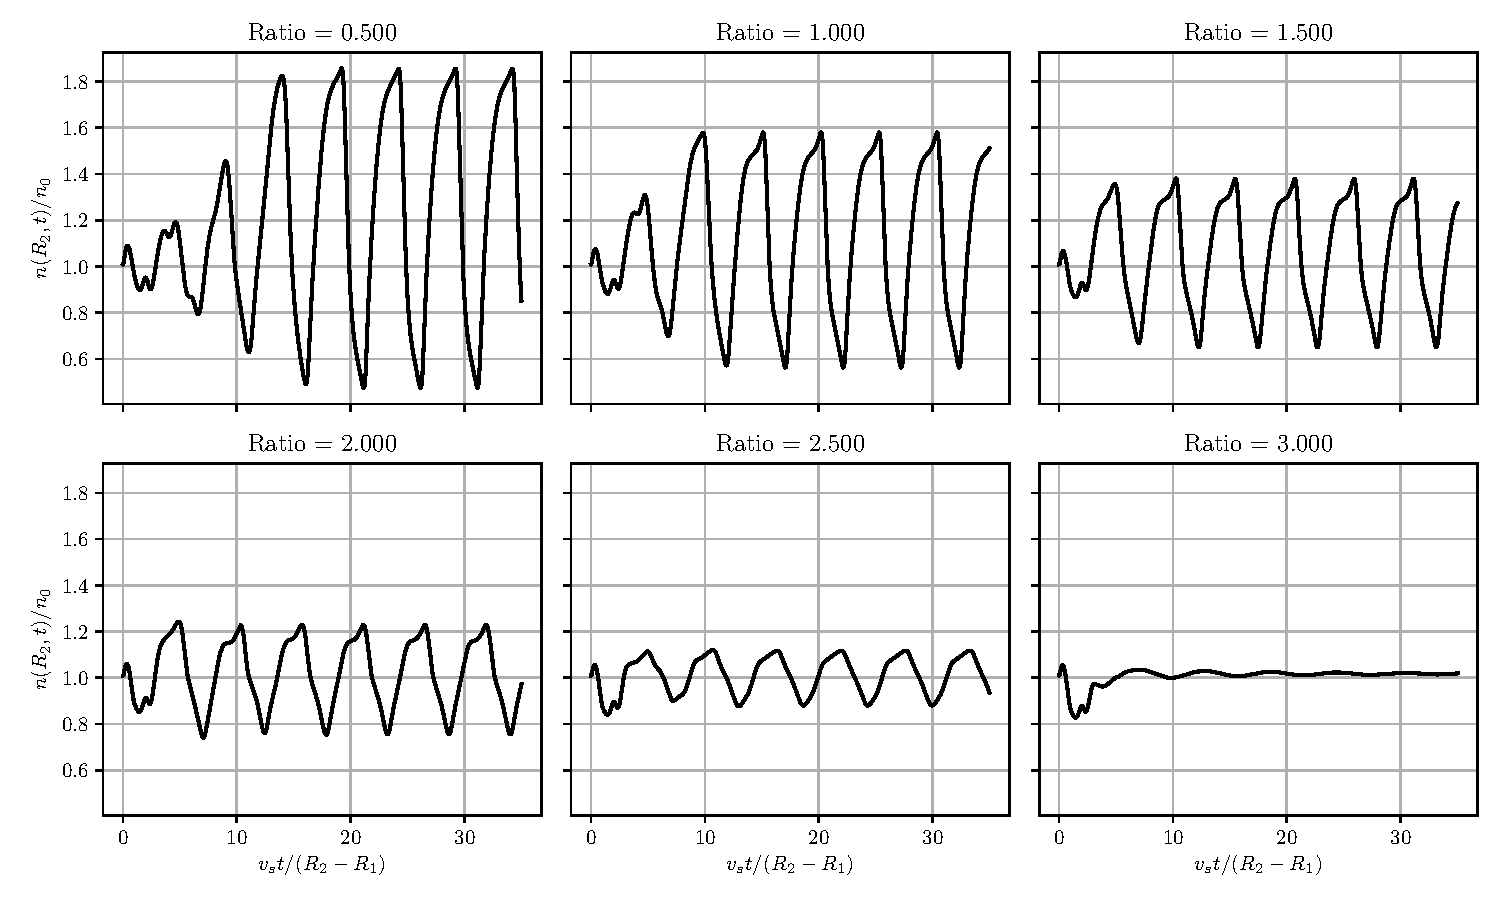
\includegraphics[width=\textwidth]{Figures/varyRatio.pdf}
			\caption{Changing ratio $(R_2 - R_1) / R_1$ at parameter values $v_0 = 0.14$, $\eta = 0.01$, $\gamma = 0.04$.}\label{fig:varyRatio}
		\end{figure}
	And Fig. \ref{fig:frequencyRatio} shows the change in frequency (in non-dimensional units as well) as the ratio is decreased.
	\begin{figure}[H]
		\centering
		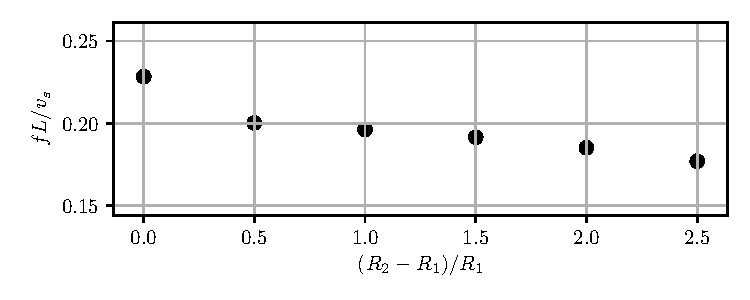
\includegraphics[width = 0.75\textwidth]{Figures/frequencyRatio.pdf}
		\caption{Frequency $f$ v.s. $(R_2 - R_1) / R_1$}\label{fig:frequencyRatio}
	\end{figure}
	Finally, Fig. \ref{fig:varyRatioSnapshots} shows the dynamics of $n$ and $J$ over the period of the oscillator at the relatively high value $(R_2 - R_1) / R_1 = 2.500$.  I don't really know what to make of this --- it looks a little wonky.  The ``bump" in $n$ could come from the presence of a bunch of terms that are much stronger at lower values of $r$ I'm not sure.
	
	I'm a bit worried about the boundary conditions' being obeyed everywhere --- the $J$ trace, in particular, looks like it's having trouble with the Neumann condition at $r = R_1$. Need to double check everything. 
	\begin{figure}[H]
		\centering
		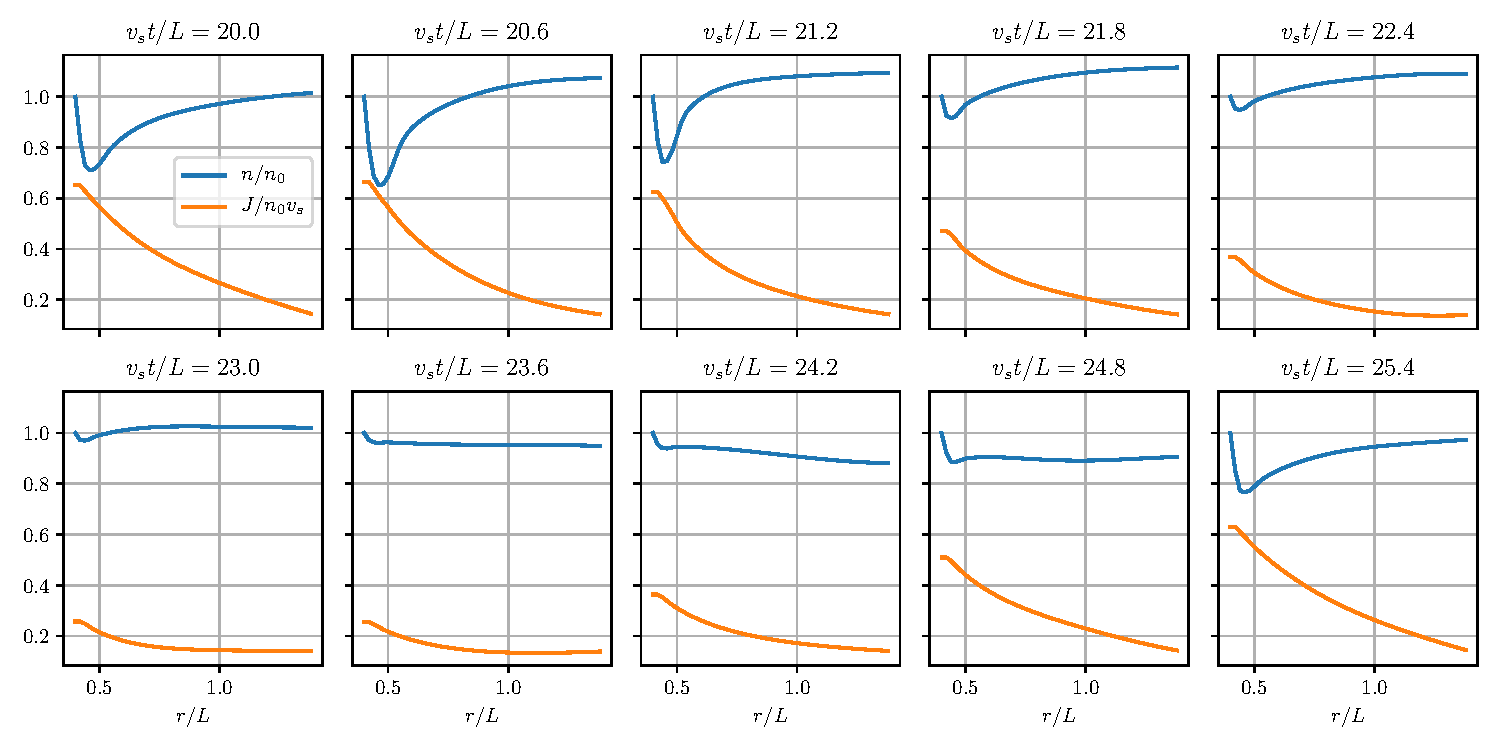
\includegraphics[width=\textwidth]{Figures/varyRatioSnapshot.pdf}
		\caption{Snapshots of $J$ and $n$ at $(R_2 - R_1) / R_1 = 2.500$}\label{fig:varyRatioSnapshots}
	\end{figure}
	
	\subsection{Parameter Space Investigations}
	In Mendl et al., they talk about how increasing $v_0$ always makes the frequency go down.  I want to check if this was also true in the polar coordinates --- in particular, is there a value of the ratio $(R_2 - R_1) / R_1$ where increasing the bias current ($v_0$) also increases the frequency?  Equally, is there a value of $v_0$ or $\eta$ where increasing that ratio actually increases the frequency or the amplitude? Basically, I'm trying to use $(R_2 - R_1) / R_1$ as another parameter that can be varied in an experimental setup to try and maximize the frequency of the oscillator.  It's doubtful that increasing this ratio will ever increase the frequency, but I guess you never know and it's worth exploring.  Does that make any sense?
		 
\end{document}